\chapter{Code Analysis AIs}

Code Analysis AI tools are Ai-based development tools designed to aid developers in evaluating their code in order to detect potential problems and suggest corrections. Unlike Code Generating AIs, these tools focus on analyzing and reviewing code that's already been written instead of generating their own. Their goal is to support software quality with bug-detection, enforcing coding standards, and bringing up areas that could affect maintainability or security.

The use of these tools has been increasing in recent years, this is due to software systems becoming more complex and harder for humans \textit{alone} to maintain. These AIs reduce human efforts by automating some of the review and analysis process while still providing feedback. Even so, their effectiveness depends on the accuracy of the analysis they provide and on how programmers interpret it and apply the corrections.

This chapter gives an overview of code analysis AI tools and discusses some selected systems such as Qodo, CodeRabbit, and CodeAnt AI. The analysis focuses on their main functionalities, modes of integration, and their impact on software quality.

\newpage

\begin{table}[h]
\small
\centering
\caption{Feature-based comparison of selected Code Analysis AIs}
\resizebox{1\textwidth}{41pt}{
\begin{tabular}{|c|c|c|c|}
\hline
\textbf{Feature} & \textbf{Qodo} & \textbf{CodeRabbit} & \textbf{CodeAnt AI}\\
\hline
\textbf{Primary purpose} & Automated code review & Code quality assessment & AI-driven code analysis \\
\hline
\textbf{Type of analysis} & Static code analysis & Static with quality metrics & Static with machine learning techniques \\
\hline
\textbf{Bug detection} & Detection of common bugs & Detection of bugs \& code patterns & Detection of bugs \& anomalous code patterns \\
\hline
\textbf{Integration environment} & IDEs \& pull requests & IDEs \& repository platform & IDE focused \\
\hline
\textbf{Feedback timing} & Post-analysis review & Post-analysis review & Real-time feedback \\
\hline
\textbf{Security-related analysis} & Limited focus & Not primary focus & Detection of security issues \\
\hline
\textbf{Refactoring support} & Limited \& descriptive & Explicit suggestions & Automated \& context-aware suggestions \\
\hline
\textbf{Use of Machine Learning} & Rule based \& ML-assisted analysis & ML assisted analysis & ML assisted analysis \\
\hline
\end{tabular}
}
\label{table_4.1}
\end{table}

Table \ref{table_4.1} shows how AI code analysis tools are differentiated, not just by their functional scope but also by the level of automation and by the role that machine learning plays in the review process. 

\section{Qodo}

Founded in 2022 with the name \textbf{Codium}, Qodo's main focus is to make sure the code quality in multi-repo environments is enforced, so that bigger teams manage to ship software faster and more reliably\cite{qodo}. It's mainly designed for organizations in which multiple programmers work on complex databases.

Qodo works by using AI to provide deep and thorough code analysis during the whole development of a piece of software by being innately integrated in the programmer's IDE and pull requests. It can learn company standards and align its recommendations with the company conventions once it has received enough information on what its expected or needed.

Software quality wise, Qodo helps improve the maintainability and reliability of the source code. It helps reducing technical debt and promotes uniform coding practices by analyzing how the code is modified and by constantly enforcing standards, so that issues can be addressed before deployment and end up with a more stable end-result.

On the other hand, programmers need to keep validating the recommendations that Qodo gives for them to be effective, this reinforces the importance of humans reviewing code analysis AIs.

\newpage

\section{CodeRabbit}

Founded in early 2023, CodeRabbit's purpose is to aid developers to find mistakes in their programs, it achieves this by scanning the source code, find bugs, suggest solutions, and elaborate on possible consequences if something is not fixed. Once it's in a programmer's cycle it can access and review pull requests, help a team review code and ship pieces of software faster, with fewer bugs making it in the final product\cite{CodeRabbit}. 

\begin{figure}[H]
    \centering
    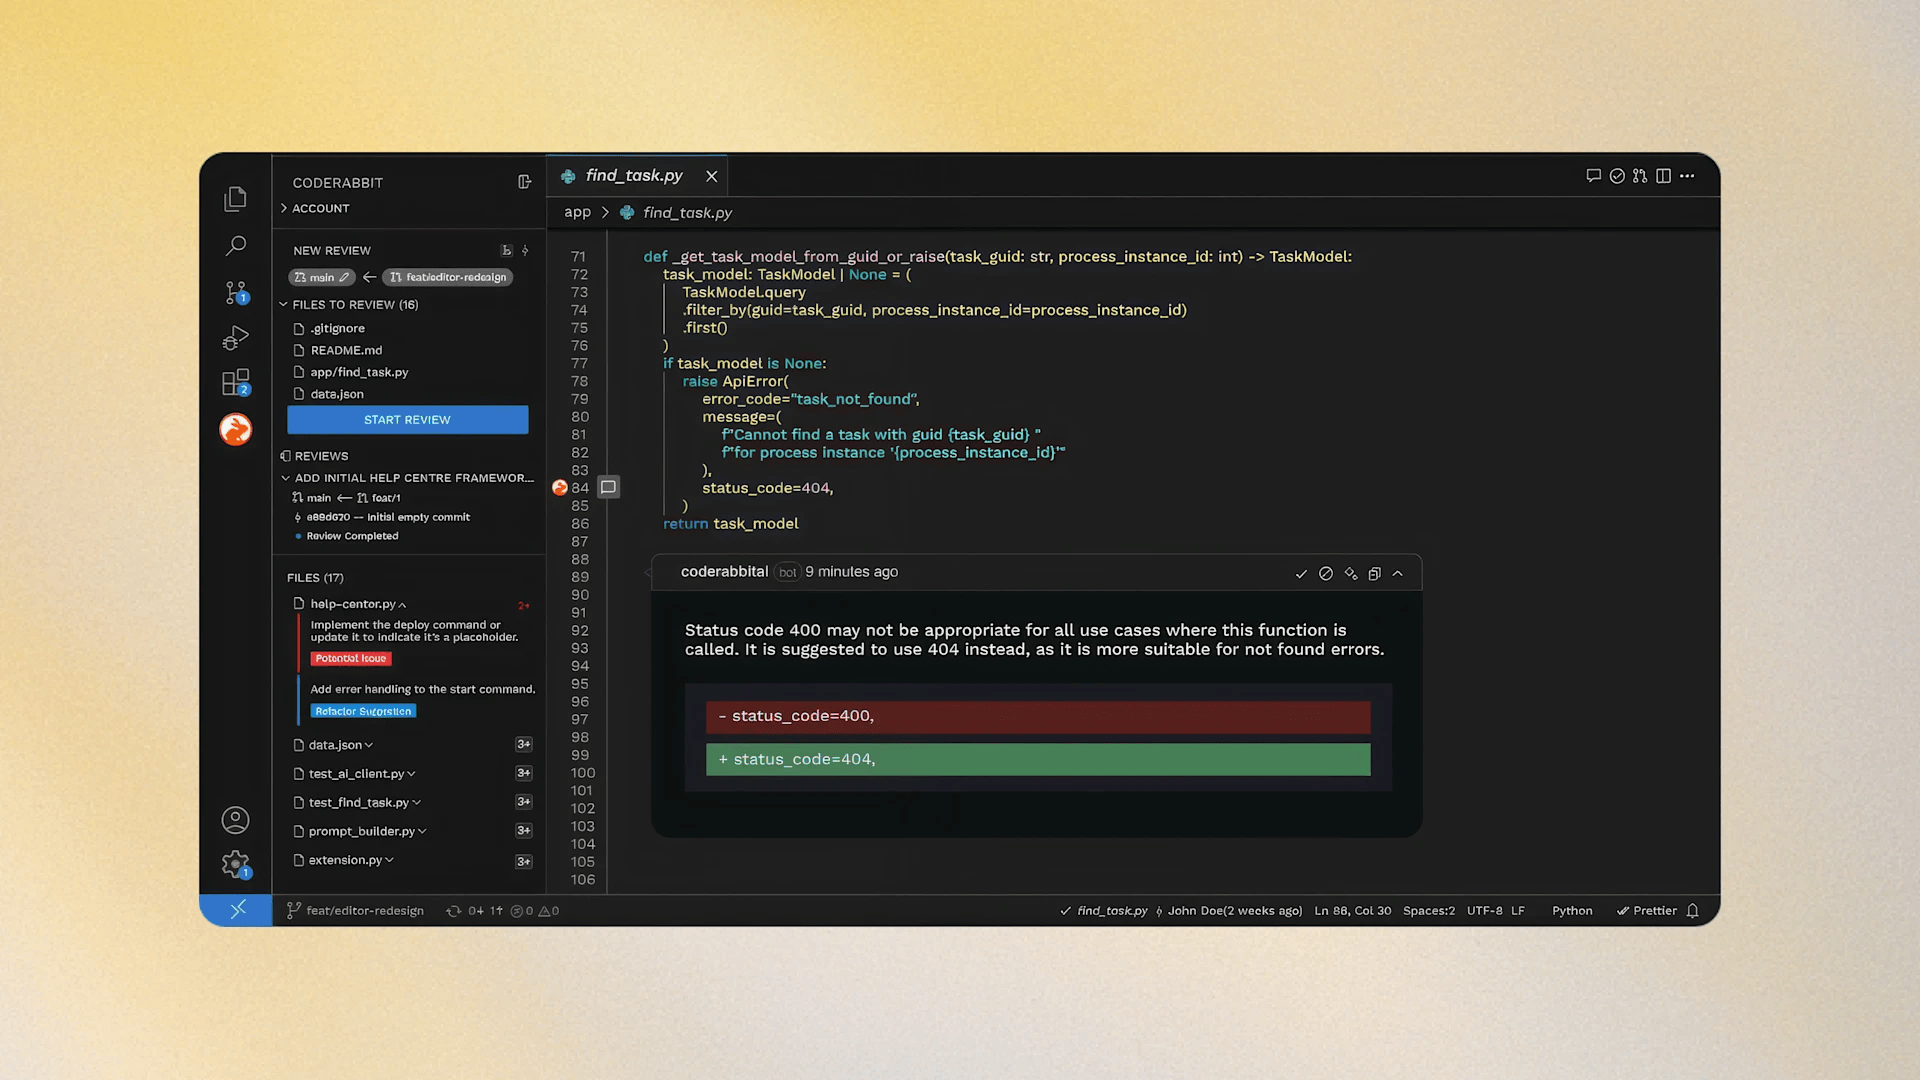
\includegraphics[width=1.081\linewidth]{images/oai_Coderabbit_UI_asset_16x9.png}
    \caption{CodeRabbit suggestion in IDE\cite{coderabbit_ui}}
    \label{fig:coderabbit_1}
\end{figure}

CodeRabbit uses AI to analyze ho source code changes in various pull requests, allowing for feedback to be provided beyond simple syntax. The suggestions it offers are accompanied by explanations, helping developers get a better understanding behind both the issues and the solutions.

In software quality terms, it helps identifying bugs early in the programming cycle, this tool reduces the chances of having faulty code being merged in the main branches of a program. In addition to that, the emphasis on contextual feedback can help development teams share knowledge, leading to better programming practices over time.

Nevertheless, just like with various code analysis AIs, the responsibility of accepting or not the various suggestions \textit{always} remains with the humans overlooking the tool.

\section{CodeAnt AI}

CodeAnt was founded as software startup in 2023 San Francisco, California\cite{CodeAnt}. It's designed to help developers identify the quality and safety issues inside the code. It's purpose is to analyze codebases and to find vulnerabilities, bugs, and structural problems that may affect maintainability. Unlike code generating tools, CodeAnt AI focuses on improving the quality of a piece of software by evaluating and refining already written code.

\begin{figure}[H]
    \centering
    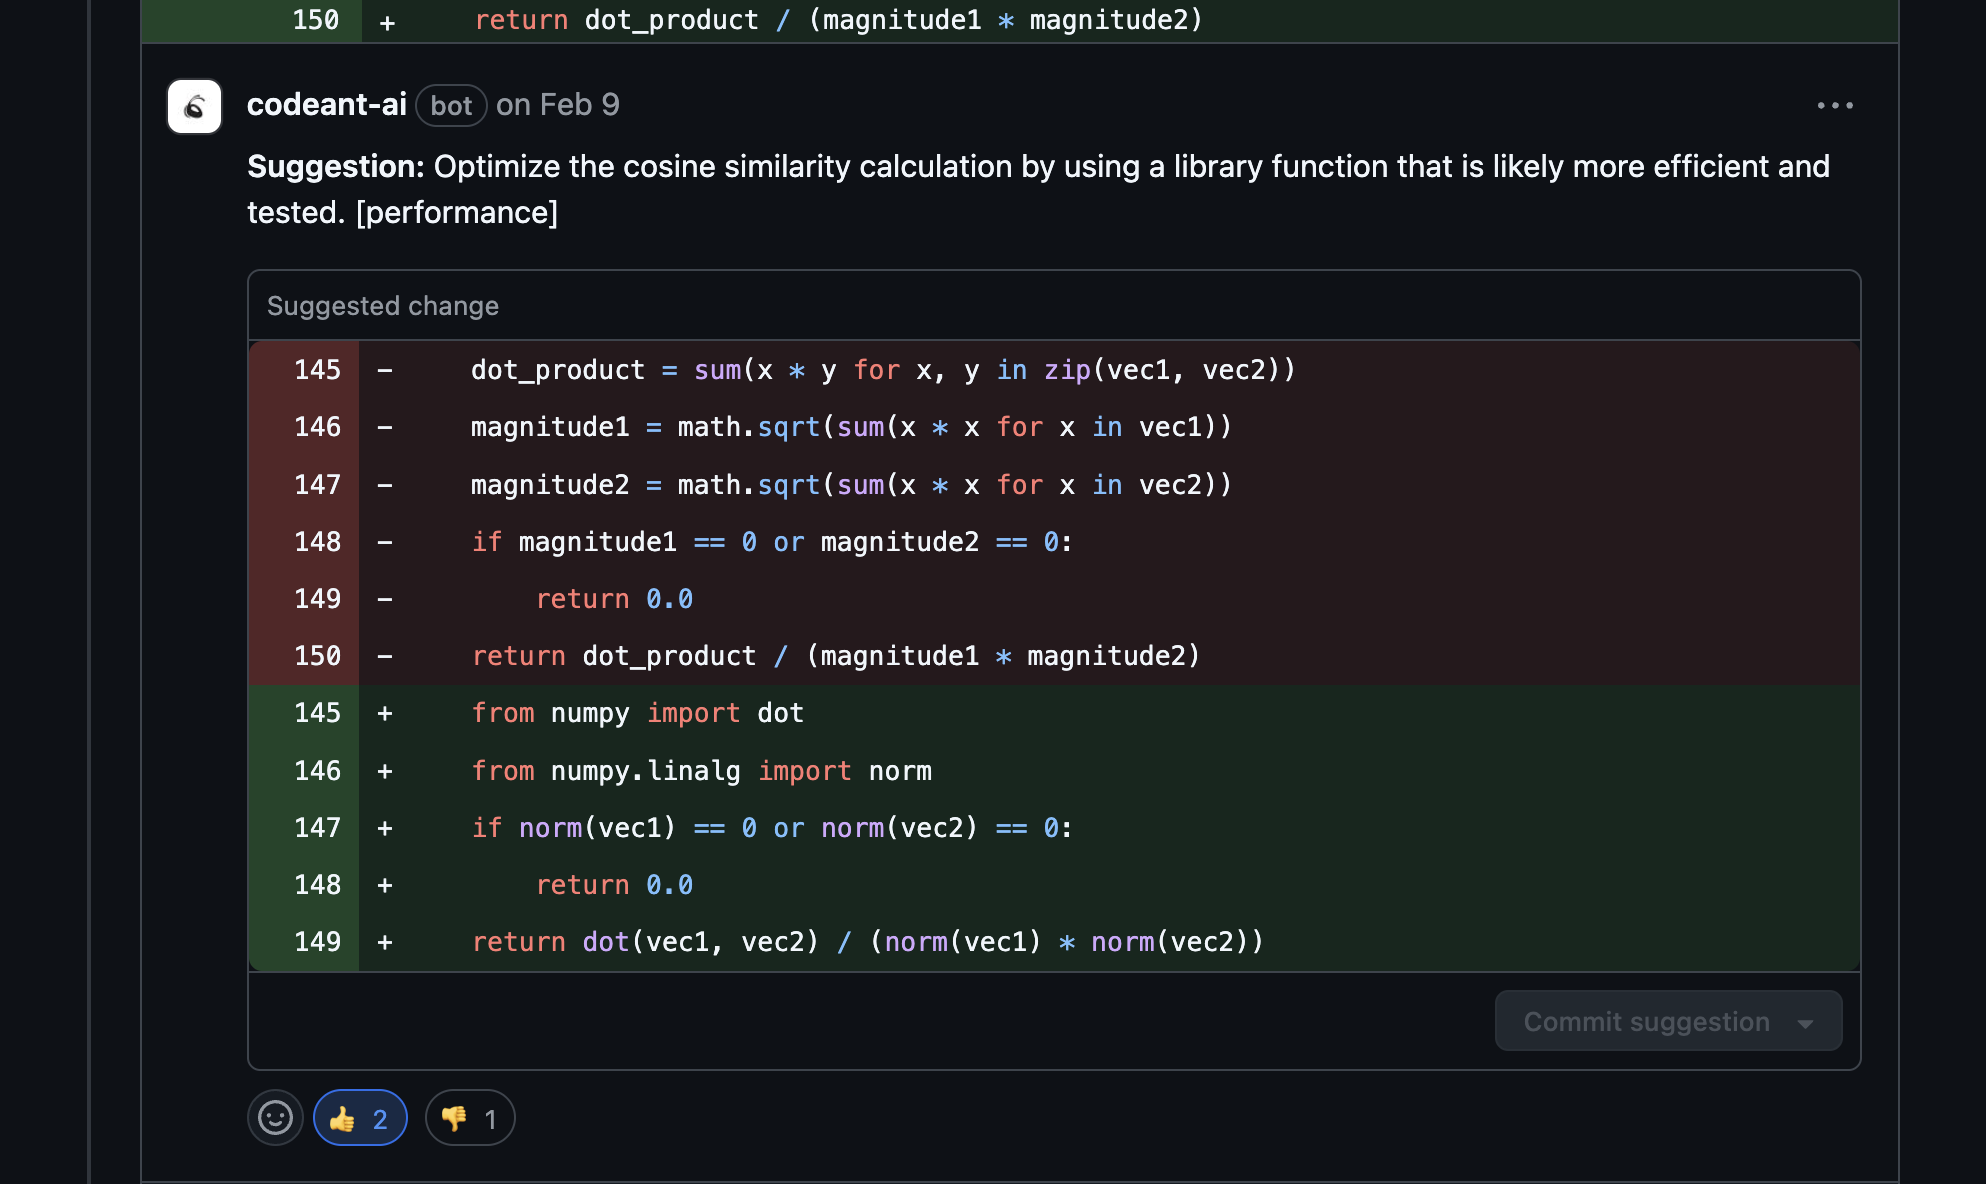
\includegraphics[width=0.9\linewidth]{images/ai-code-review-in-action.png}
    \caption{CodeAnt suggestion in IDE\cite{codeant_ui}}
    \label{fig:codeant_1}
\end{figure}

CodeAnt main concerns are software security and maintainability. Through an automated analysis, it shows weaknesses that be the reasons behind security problems or technical debt if left unattended. Because of this, especially when its done in the early stages of programming, the tool becomes important when reliability and compliance are a major goal and it also help developers maintain a cleaner and sustainable code structure in the long run.

When analyzed from a software quality point of view, CodeAnt's objective is to improve the maintainability and structure of a program, the detection of problems in the early stages lets teams fix them before they propagate throughout the system.

However, even in this case human intervention is still required when interpreting and validating CodeAnt's suggestions, reinforcing the programmers' role in quality decisions and making the final design.